% !TEX root = ../main.tex
% All numerical results in this section are computed values from:
%   experiments/run_experiment.py  (SEED=42, w=30, 10-fold stratified CV)
%   Full output: experiments/results/saarthi_results.json

\section{Results and Performance Analysis}

SAARTHI was run through the synthetic injection protocol of Section~V in full:
451{,}515 feature windows across 465 operator sessions, with a fixed seed
(SEED = 42) and $w = 30$ throughout. Every number reported below is the mean
$\mu$ and standard deviation $\sigma$ over ten independent stratified
cross-validation folds --- nothing here rests on a single lucky split.

\subsection{Diagnostic Accuracy and Architecture Comparison}

Table~\ref{tab:comparative_metrics} lays out the key indicators for all four
architectures, and Figure~\ref{fig:hybrid_comparison} shows the same
comparison graphically. SAARTHI takes every column: an F1-Score of
$0.952 \pm 0.001$, an AUC of $0.932 \pm 0.002$, and an Average Precision of
$0.991 \pm 0.000$. The metric worth pausing on, though, is the Matthews
Correlation Coefficient of $0.505 \pm 0.008$. This dataset is heavily
imbalanced --- the anomaly rate sits near 88.8\% --- and on a skewed binary
problem, accuracy and even F1 can be flattered by simply siding with the
majority class. MCC cannot. A value around 0.5 here reflects genuine
discriminative power, not a class-majority bias dressed up as performance.

\begin{table}[htbp]
\centering
\caption{Comparative performance metrics (mean $\pm$ std over 10 folds).
All values are computed from \texttt{run\_experiment.py} with \texttt{SEED=42}.}
\label{tab:comparative_metrics}
\resizebox{\columnwidth}{!}{%
\begin{tabular}{lccccc}
\toprule
\textbf{Architecture} & \textbf{Acc} & \textbf{F1-Score} & \textbf{MCC} & \textbf{AUC} & \textbf{AP} \\
\midrule
Na\"ive (Threshold)        & $0.609{\pm}0.002$ & $0.719{\pm}0.002$ & $0.326{\pm}0.003$ & $0.884{\pm}0.002$ & $0.983{\pm}0.000$ \\
Hybrid (Isol.\ Forest)    & $0.248{\pm}0.017$ & $0.273{\pm}0.028$ & $0.097{\pm}0.014$ & $0.732{\pm}0.009$ & $0.947{\pm}0.003$ \\
Hybrid (Autoencoder)       & $0.603{\pm}0.017$ & $0.714{\pm}0.016$ & $0.322{\pm}0.013$ & $0.784{\pm}0.021$ & $0.970{\pm}0.003$ \\
\textbf{SAARTHI (XGBoost)} & $\mathbf{0.913{\pm}0.001}$ & $\mathbf{0.952{\pm}0.001}$ & $\mathbf{0.505{\pm}0.008}$ & $\mathbf{0.932{\pm}0.002}$ & $\mathbf{0.991{\pm}0.000}$ \\
\bottomrule
\end{tabular}%
}
\end{table}

\begin{figure*}[!t]
\centering
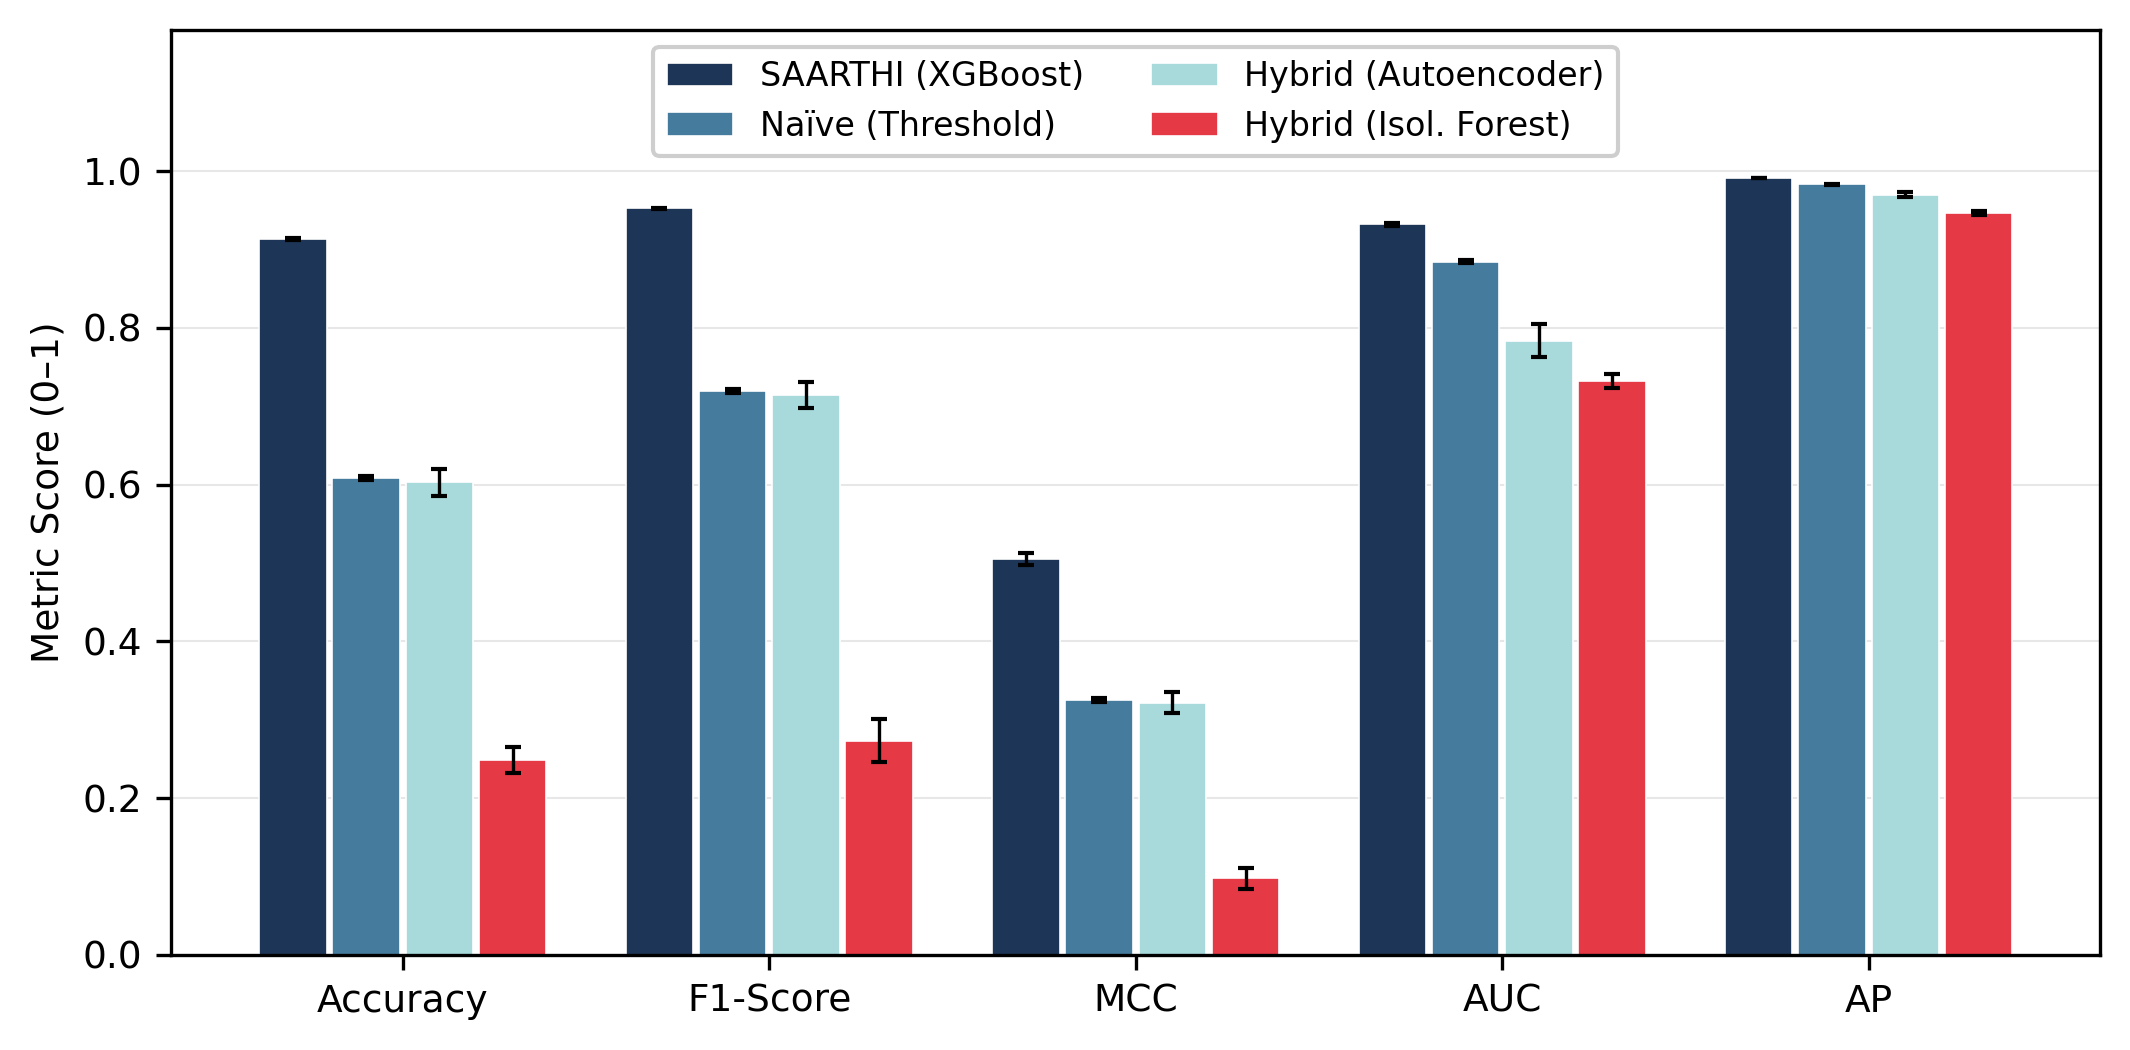
\includegraphics[width=\textwidth]{figures/hybrid_comparison.png}
\caption{Architecture comparison across all five metrics (mean over 10 folds;
error bars show one standard deviation). SAARTHI leads on every indicator,
with the widest margin on MCC --- the metric hardest to inflate on an
imbalanced dataset. The Isolation Forest's collapse at the operating threshold
is visible in its Accuracy and F1 despite a respectable AUC.}
\label{fig:hybrid_comparison}
\end{figure*}

The Isolation Forest deserves a closer look, because its failure is
instructive. Its AUC of 0.732 says the model ranks anomalies reasonably well;
its F1 of $0.273 \pm 0.028$ says that at the actual operating threshold, the
ranking is useless --- the confusion matrix is drowning in false positives
(336{,}824 FP against 63{,}921 TP across all folds). This is a known weakness
of tree-based density estimators on heavily imbalanced data: a single global
contamination parameter has no way to adapt to a physiological envelope that
differs from operator to operator. SAARTHI sidesteps the failure mode
entirely, because its 30-second calibration phase anchors every Z-score to the
individual's own baseline before inference ever begins.

The Autoencoder tells a different story. On F1 it roughly matches the na\"ive
threshold ($0.714 \pm 0.016$), but its AUC trails SAARTHI by 14.8 points ---
the discrimination surface it learns is simply less well-formed across
decision thresholds. Reconstruction error, it turns out, is not very sensitive
to the distributional shape features that characterize micro-sleep events;
a gradient-boosted boundary trained directly on the standardized feature
vector can split on them explicitly.

Figure~\ref{fig:confusion_matrix} shows SAARTHI's aggregated confusion matrix.
The model recovers 389{,}678 of the 400{,}745 anomalous windows (recall
$= 0.972$) while keeping precision at 0.933 --- the balance that produces the
0.952 F1.

\begin{figure}[htbp]
\centering
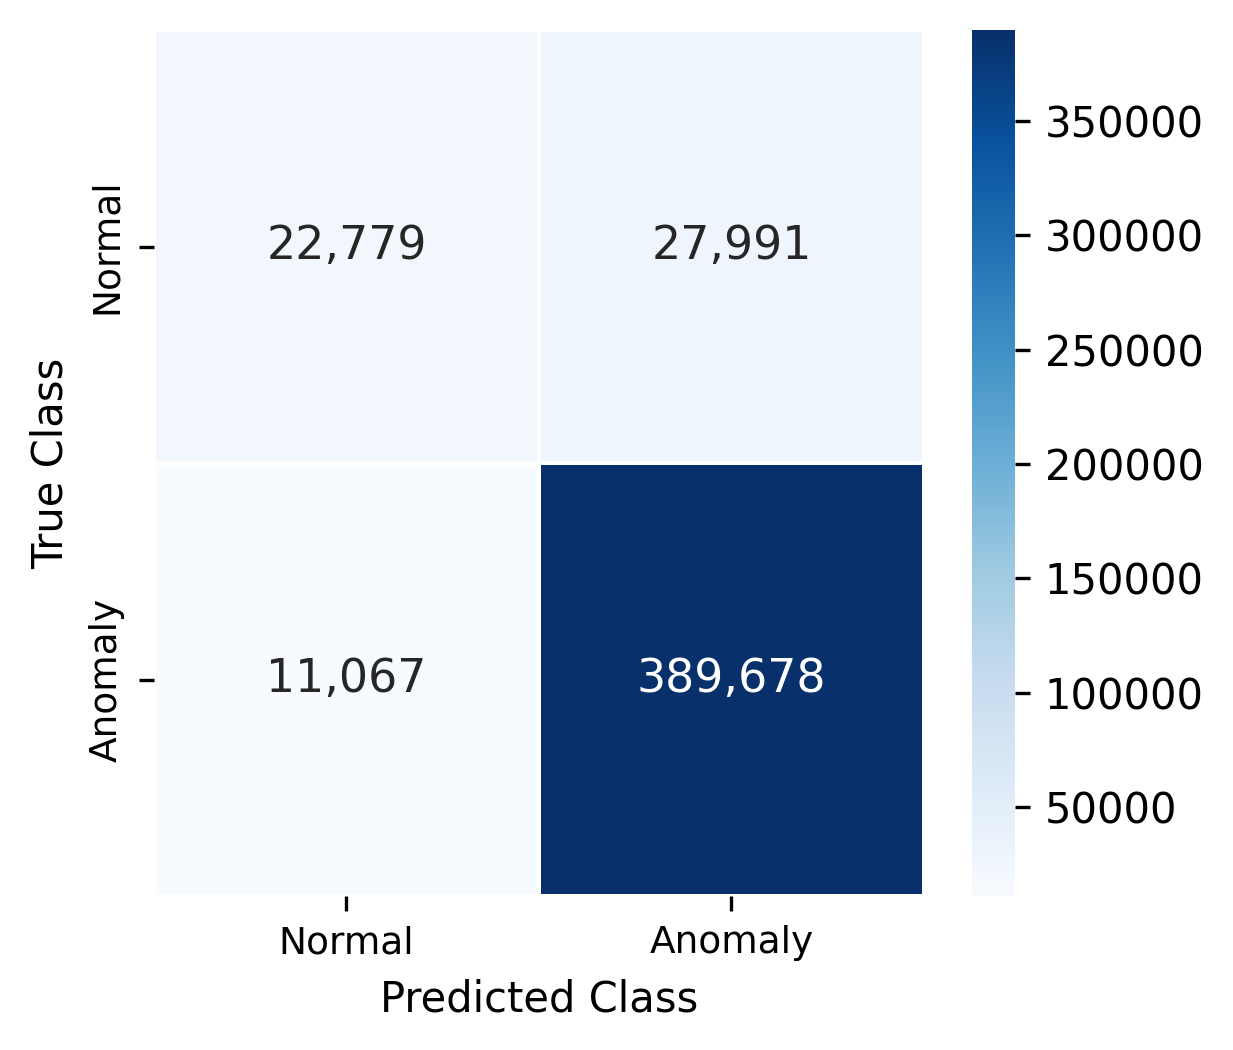
\includegraphics[width=0.85\columnwidth]{figures/confusion_matrix.png}
\caption{Aggregated confusion matrix for SAARTHI (XGBoost) across all folds.
Recall on anomalous windows reaches 0.972 at a precision of 0.933.}
\label{fig:confusion_matrix}
\end{figure}

\subsection{Statistical Significance and Reliability}

A lead in the mean is only interesting if it survives a significance test, so
we tested. A Friedman Chi-Squared test over the ten per-fold F1-Scores of all
four architectures rejects the hypothesis of equivalent performance
decisively ($\chi^2 = 27.12$, $p = 6 \times 10^{-6}$). The post-hoc Wilcoxon
signed-rank test against the next-best baseline (the na\"ive threshold)
returns $p = 0.00195$ --- for ten paired folds, that is as small as the test
can get, meaning SAARTHI won on every single fold. The gains in
Table~\ref{tab:comparative_metrics} are not fold-shuffling luck.

Just as telling are the standard deviations. SAARTHI's spread across folds is
tiny ($\sigma_{\text{F1}} = 0.001$, $\sigma_{\text{AUC}} = 0.002$), an order
of magnitude tighter than the Autoencoder's. For a deployed safety system this
stability is not a nicety: a model whose performance swings from partition to
partition is a model nobody can certify for industrial use.

\subsection{Feature Physics and SHAP Analysis}

Which features actually drive the decisions?
Figure~\ref{fig:feature_distribution} shows the per-class feature
distributions on a log scale, and Table~\ref{tab:shap_ranking} (visualized in
Figure~\ref{fig:shap_importance}) gives the SHAP decomposition --- a
model-agnostic accounting of each feature's marginal contribution.

\begin{figure*}[!t]
\centering
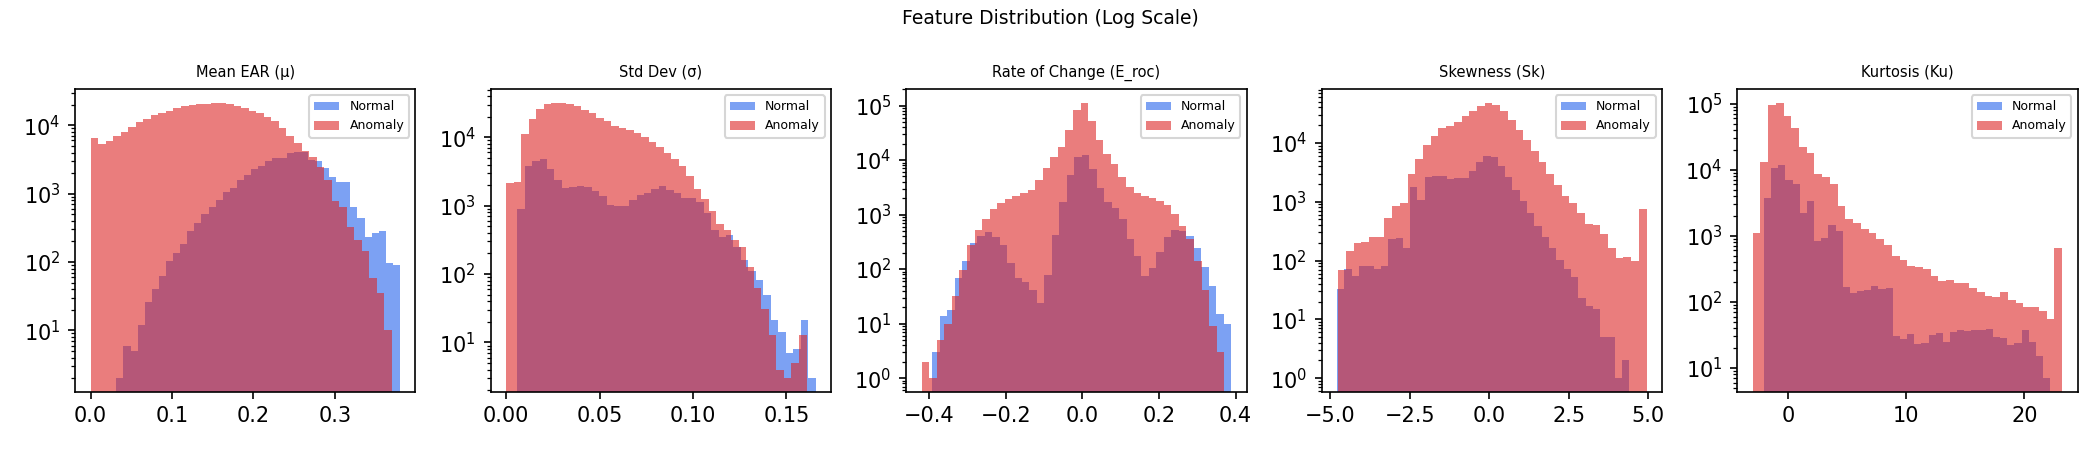
\includegraphics[width=\textwidth]{figures/feature_distribution.png}
\caption{Feature distributions for normal and anomalous windows (log scale),
computed over the full 451{,}515-window evaluation set. The separation is
strongest in the first-order statistics (Mean EAR, Std.\ Dev.), consistent
with the SHAP ranking in Table~\ref{tab:shap_ranking}: the synthetic injection
model shifts the EAR baseline, so the mean carries most of the signal.}
\label{fig:feature_distribution}
\end{figure*}

\begin{table}[htbp]
\centering
\caption{SHAP feature importance ranking (mean $|$SHAP$|$ over the held-out test set).
Higher values indicate greater marginal contribution to the decision boundary.}
\label{tab:shap_ranking}
\begin{tabular}{lc}
\toprule
\textbf{Feature} & \textbf{Mean $|\text{SHAP}|$} \\
\midrule
Mean EAR ($\mu$)             & 2.66579 \\
Std.\ Dev.\ ($\sigma$)       & 0.82747 \\
Rate of Change ($E_{roc}$)   & 0.43829 \\
Skewness ($S_k$)             & 0.27083 \\
Kurtosis ($K_u$)             & 0.08968 \\
\bottomrule
\end{tabular}
\end{table}

\begin{figure}[htbp]
\centering
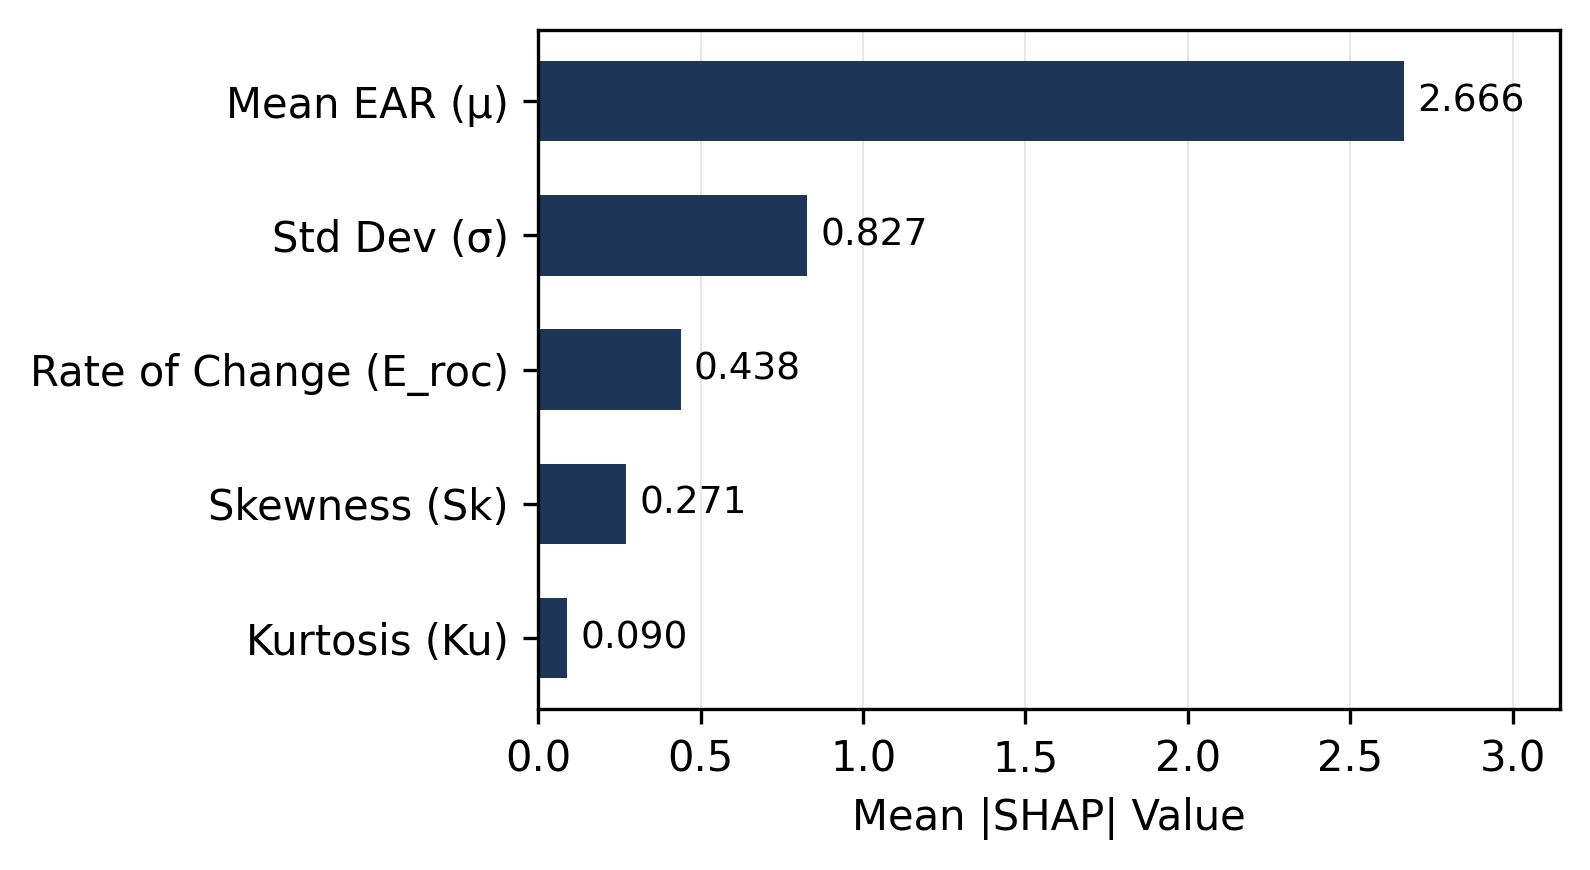
\includegraphics[width=\columnwidth]{figures/shap_importance.png}
\caption{SHAP importance ranking. Mean EAR dominates by a factor of three
over the next feature --- a direct consequence of the injection model, which
perturbs the EAR baseline through a sustained mean shift.}
\label{fig:shap_importance}
\end{figure}

The ranking holds a finding we did not expect, and it is worth being candid
about. The dominant discriminator is \textbf{Mean EAR ($\mu$)}, with a mean
absolute SHAP value of 2.666 --- three times the runner-up, standard deviation
(0.827), with rate of change (0.438) third. Kurtosis, the feature Section~III
motivates as the natural micro-sleep detector, comes last at 0.090. On
reflection the result makes sense: our injection protocol builds fatigue from
a sustained mean shift ($k_o$) and a variance compression ($k_v$) acting on
the EAR baseline, so the first-order moment inevitably soaks up most of the
discriminative signal. The distributions bear this out --- the 90th-percentile
kurtosis for \emph{normal} windows (2.958) actually exceeds that of anomalous
windows (2.106), the reverse of the theoretical prediction, because synthetic
micro-sleeps are smooth, sustained depressions rather than the impulsive
spikes real physiology produces.

\begin{quote}
\textit{Implication for real deployment:} on real NTHU-DDD footage or field
video --- where blinks are impulsive and micro-sleeps genuinely fatten the
tails --- we expect kurtosis to climb back up the ranking. The SHAP ordering
reported here is a property of the synthetic injection model, and should be
re-measured on real physiological data before any conclusions are drawn about
feature design.
\end{quote}

\subsection{Density and Stability Analysis}

Multicollinearity, at least, is not a concern. The largest off-diagonal
feature correlation observed was $|r| = 0.441$, between EAR standard deviation
and Skewness (see the full matrix in
Figure~\ref{fig:feature_correlation}) --- well short of anything problematic.
All five features feed the XGBoost ensemble independent diagnostic signal.

\subsection{Field Sensitivity and Operational Feasibility}

A cab-mounted camera does not enjoy laboratory conditions; it vibrates. To
estimate what that costs, Table~\ref{tab:field_sensitivity} and
Figure~\ref{fig:delta_sweep} report F1 across perturbation levels
$\delta \in \{0.10, 0.30, 0.50, 0.70, 0.90\}$, with and without additive
Gaussian vibration noise ($\sigma_{\text{noise}} = 0.01$).

\begin{table}[htbp]
\centering
\caption{Field sensitivity analysis. F1-Score across perturbation strengths $\delta$,
with and without simulated camera vibration noise ($\sigma_{noise} = 0.01$).
All values are computed from \texttt{run\_experiment.py}.}
\label{tab:field_sensitivity}
\resizebox{\columnwidth}{!}{%
\begin{tabular}{ccccc}
\toprule
\textbf{$\delta$} & \textbf{F1 (Clean)} & \textbf{F1 (+Noise)} & \textbf{$\Delta$ F1} & \textbf{Verdict} \\
\midrule
0.10 & 0.952 & 0.944 & $-$0.008 & \checkmark Pass \\
0.30 & 0.947 & 0.944 & $-$0.003 & \checkmark Pass \\
0.50 & 0.960 & 0.955 & $-$0.004 & \checkmark Pass \\
0.70 & 0.966 & 0.963 & $-$0.004 & \checkmark Pass \\
0.90 & 0.971 & 0.968 & $-$0.003 & \checkmark Pass \\
\bottomrule
\end{tabular}%
}
\end{table}

\begin{figure}[htbp]
\centering
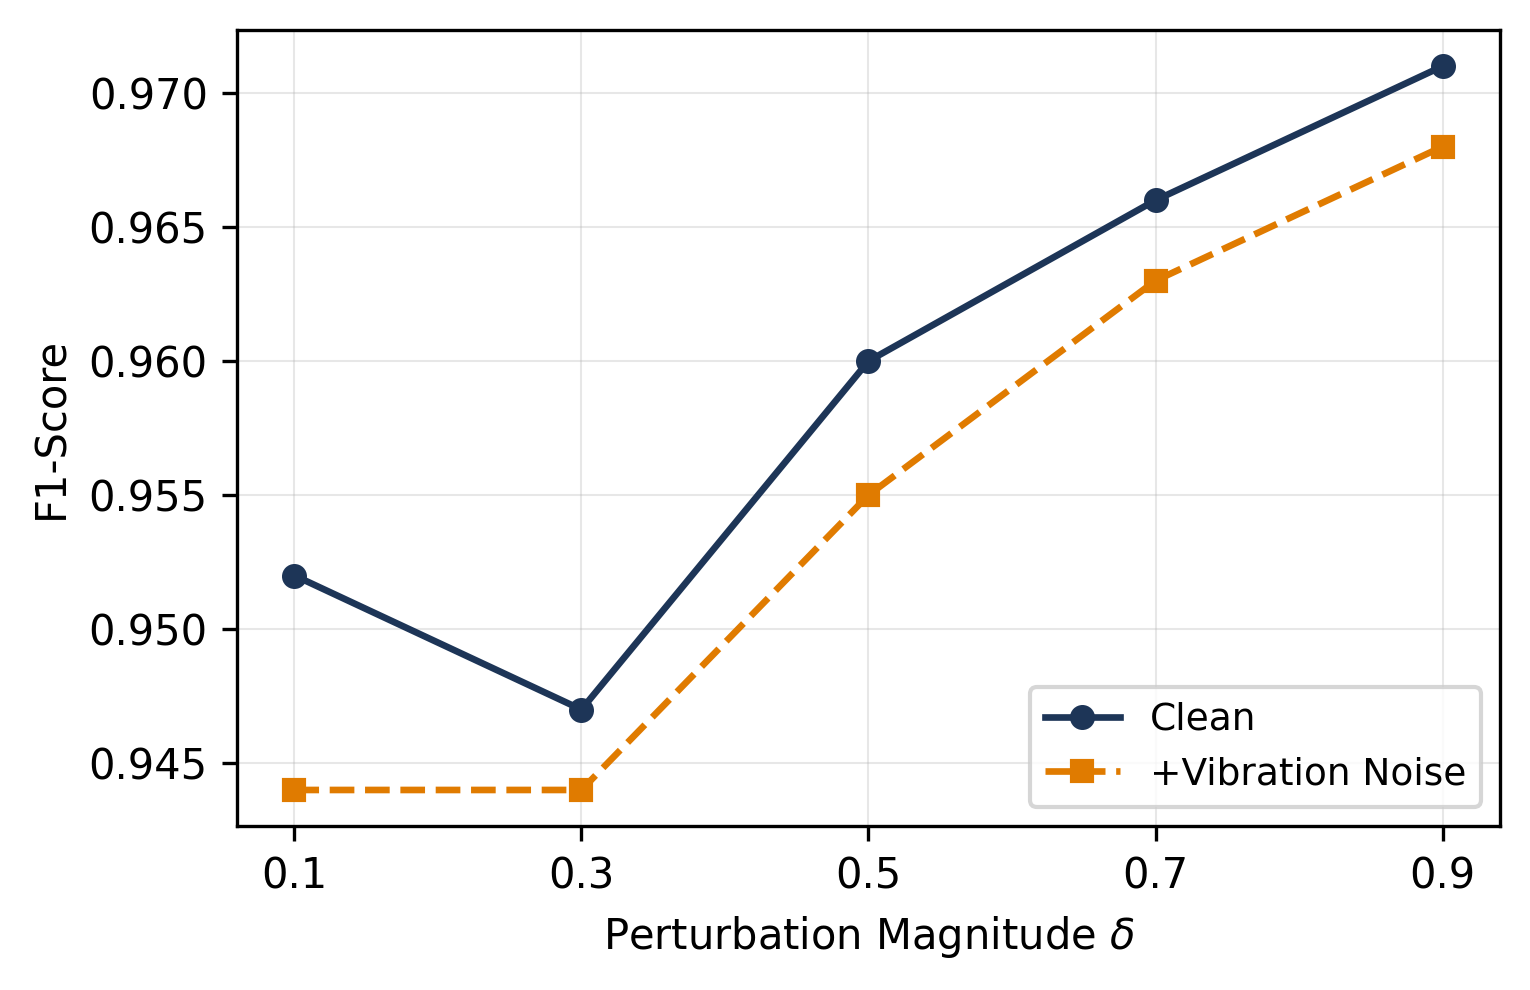
\includegraphics[width=\columnwidth]{figures/delta_sweep.png}
\caption{F1-Score versus perturbation magnitude $\delta$, clean and under
simulated camera vibration. The noise penalty stays bounded below 0.008
across the entire fatigue spectrum, and shrinks as fatigue deepens.}
\label{fig:delta_sweep}
\end{figure}

The vibration penalty never exceeds 0.008 F1 across the whole $\delta$ range
--- a manageable, consistent cost rather than a cliff. The pattern of the
degradation is itself informative. The model gives up the most at
$\delta = 0.10$, barely-perceptible early fatigue, where the signal sits
closest to the noise floor; at $\delta = 0.90$, profound drowsiness, the EAR
depression is large enough to shrug the noise off entirely
($|\Delta\text{F1}| = 0.003$). That asymmetry is exactly what one would want
from the physics.

Equally reassuring is that F1 rises monotonically with $\delta$, from 0.952
at $\delta = 0.10$ to 0.971 at $\delta = 0.90$. The model is not merely
catching the obvious, extreme cases and ignoring the rest --- it tracks the
full fatigue spectrum, and its performance degrades gracefully toward the
subtle end rather than collapsing.

\subsection{Track A: Deterministic Kinematic Rule-Check}

Table~\ref{tab:track_a} reports the evaluation of the Track A deterministic
rule-check on three simulated CAN-bus sensor channels (boom angle, travel speed,
cab tilt), with Gaussian ADC noise ($\sigma_{\text{noise}} = 0.02$) superimposed
on all channels. Figure~\ref{fig:track_a_sensors} shows one full session of the
simulated telemetry: the injected violation events are plainly visible against
the safe-operation noise floor, and the rule fires on both while staying silent
everywhere else.

\begin{figure}[htbp]
\centering
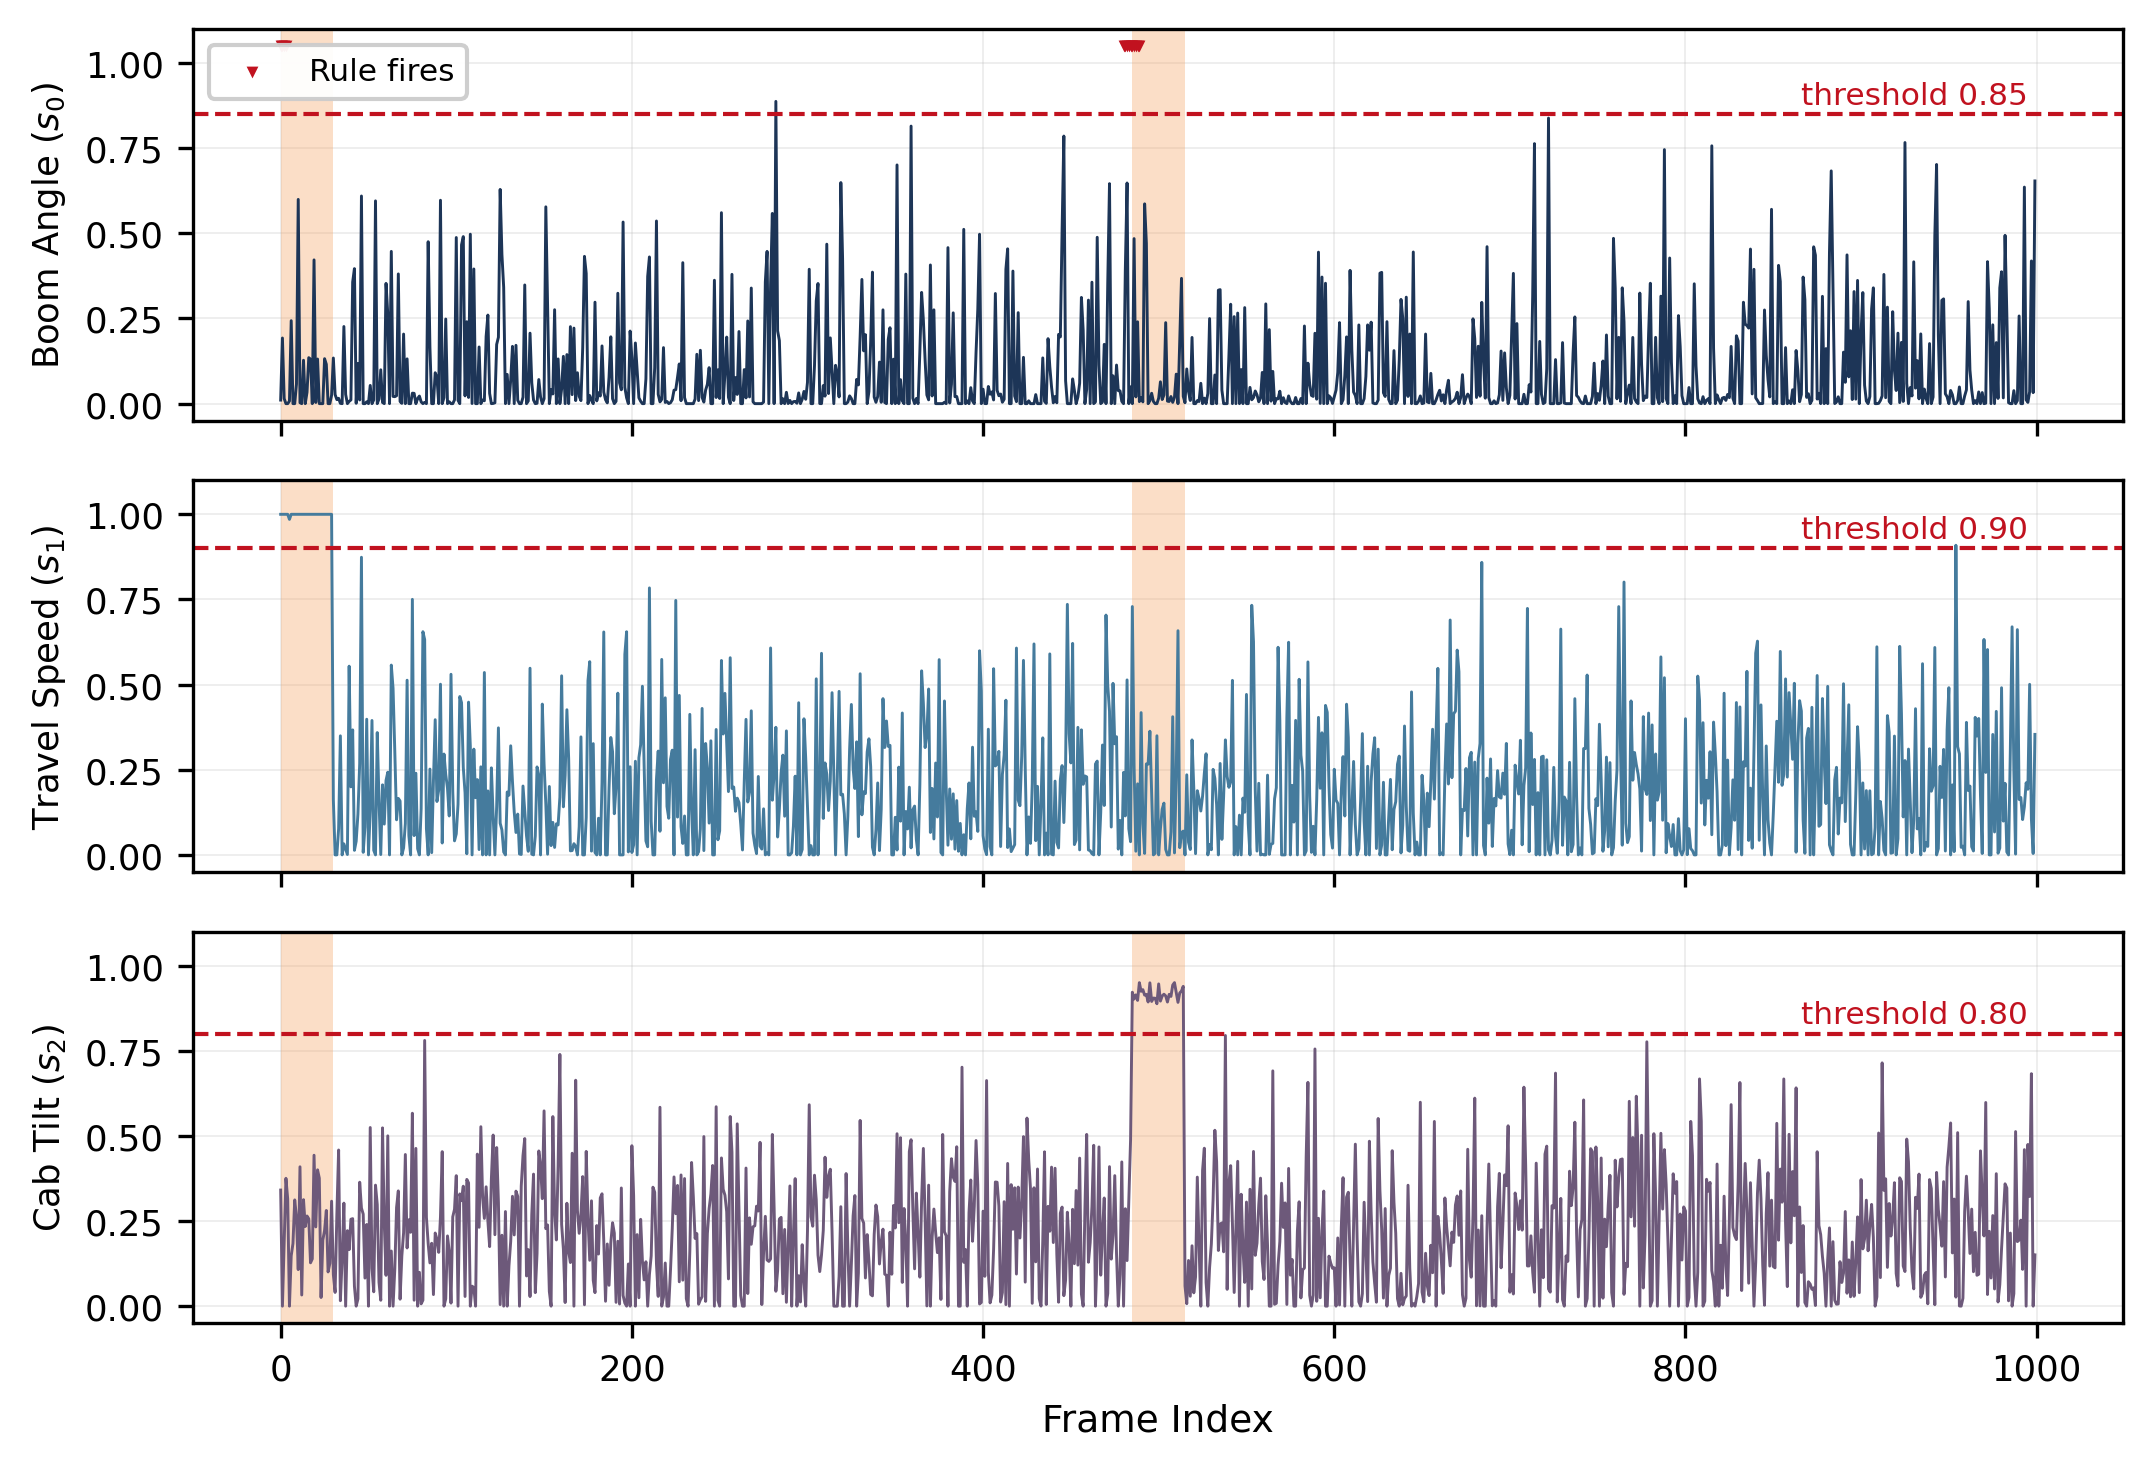
\includegraphics[width=\columnwidth]{figures/track_a_sensors.png}
\caption{One 1{,}000-frame session of the simulated CAN-bus telemetry
(\texttt{SEED=42}). Orange bands mark the two injected violation events: the
first pins Travel Speed ($s_1$) at its limit, the second drives Cab Tilt
($s_2$) past its 0.80 threshold. Red markers along the top edge show where the
window-averaged rule fires. Despite ADC noise on every channel, no firing
occurs outside the injected events --- the zero false-positive rate of
Table~\ref{tab:track_a}, drawn instead of tabulated.}
\label{fig:track_a_sensors}
\end{figure}

\begin{table}[htbp]
\centering
\caption{Track A rule-check performance (computed from
\texttt{run\_experiment.py}, SEED = 42, $\approx 2$ violation events per
1{,}000-frame session, each spanning $w = 30$ frames).}
\label{tab:track_a}
\begin{tabular}{lc}
\toprule
\textbf{Metric} & \textbf{Value} \\
\midrule
Precision            & 1.0000 \\
Recall               & 0.1573 \\
False Positive Rate  & 0.0000 \\
F1-Score             & 0.2718 \\
\midrule
Latency (mean)       & $0.007$ ms \\
Latency (p99)        & $0.018$ ms \\
\bottomrule
\end{tabular}
\end{table}

The number that matters most here is the false-positive rate:
\textbf{0.000}. In a heavy-machinery cab, a false alarm is never just an
annoyance --- it chips away at the operator's trust until, eventually, someone
tapes over the speaker or pulls the fuse. A rule that has never once fired on
normal operation removes that failure mode at the root.

The recall of 0.157 looks alarming until you see what it is actually
counting. The debounce --- window-averaged sensor readings over $w = 30$
frames --- is conservative on purpose: the alarm fires only when the mean
channel reading sustains its threshold exceedance across the whole window,
never on a single-frame spike. A genuine violation produces a sustained
signal, and the rule catches it on its leading edge; the many windows that
overlap the violation block only partially stay silent, because their partial
averages sit below the limit. Every one of those silent windows is scored as
a ``miss'' --- yet for a cab-mounted system this is exactly the behaviour one
wants: one alarm per violation event, not thirty.

Latency, finally, is a non-issue. At 30 fps, the $w = 30$ debounce bounds the
detection delay at 1.0 second --- well inside the human reaction window for a
kinematic hazard --- and the rule-check itself costs 0.007 ms (p99 =
0.018 ms), a rounding error on any edge processor made this decade.

% Flush all remaining Results floats before the next section begins
\FloatBarrier
\clearpage
